\section{Design\label{Design}}
\paragraph{}
Implementing a flexible and powerful framework for user testing of stereoscopic problems requires a design that accounts for some special requirements. To find out what those requirements are, several tests where designed and executed. The design of the application was adapted to be fit for use in those and many other imaginable tests.

\begin{figure*}[htb]
\begin{center}
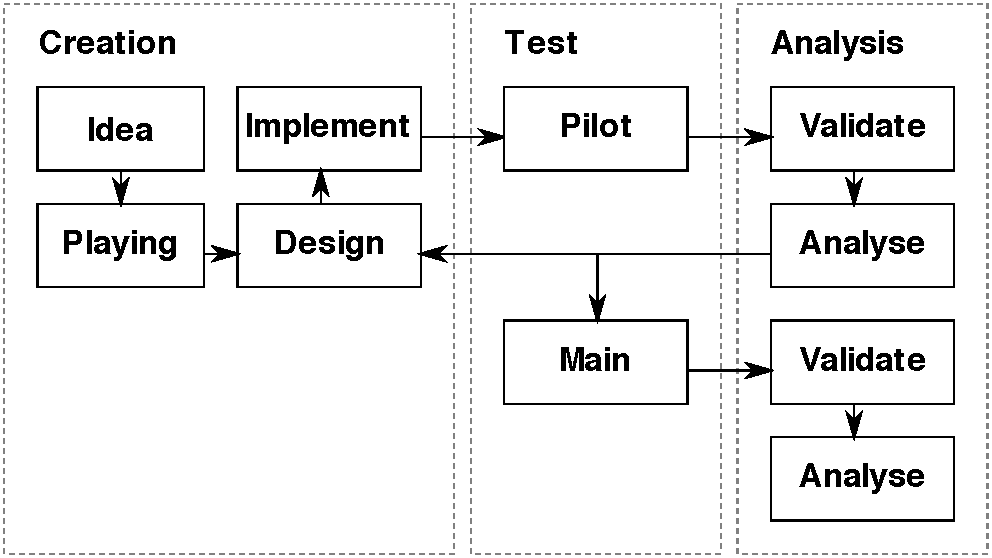
\includegraphics[width=15cm]{media/workflow.pdf}
\caption{A diagram of possible steps to create and conduct a test.\label{imgWorkflow}}
\end{center}
\end{figure*}

\paragraph{Creation}
The framework is split into three parts: The test design part aids with the construction of the test scene. A scene is a description of stimuli, possible inputs, and reactions to them. Traditional tests in this area show a series of pictures, requiring user feedback for each, while measuring the response time and the correctness. Stimuli are often precomputed and only consist of a single pixel image.

The requirements for stereoscopic test are different: It is not feasible to manually prepare stimuli, especially if complexe interaction is required. A method to generate them on the fly is needed.
Section \ref{sceneRep} describes how the look of a scene could be represented.

An important part during the creation of a scene is immediate feedback on the look of the test stimulus.
By seeing how the scene appears under test conditions, how hard it is to see, and to modify parameters with direct response,
designing a test that can be conducted by a wide range of people, and deliver reliable results is simplified.

After playing around with possible stimuli, the test has to be designed.
Now the decision which independent and dependent variables are used is made.
An other decision is the counterbalancing, the test duration, block length and many other factors.

Once the design stands, the code for the test is written.
Depending on the test, this involves counter balancing, randomisation and input validation.


\paragraph{Testing}
The testing part is the most important. It displays stimuli and logs the user replies, reacting in a way that is defined by the designer of the test. While traditional tests only follow the question-response pattern, stereoscopic user tests often require more: Trials often have to be randomized with several constraints, simply randomizing might lead to overlaps, or imbalances in dependent properties. All parameters of the stimulus have to be directly or indirectly controllable based on user input such as movement of stimuli, movement of the camera, or visibility of objects.

An other complication with stereoscopic tests is, that they have to be viewed stereoscopically.
Many methods to see stereoscopic materials exist, starting with simple color based encoding (anaglyph), over polarisation encoded frames to direct viewing of the left and right frames with special hardware.
A software for stereoscopic testing should support a wide range of output devices and methods.

Pilot tests are made to analyze if the test delivers usable results.
The main test is conducted with more subjects and possibly an improved version of the test.

\paragraph{Analysis}
Analysing the gathered data is the third part. This is usually done in a combinataion of \textit{Microsoft Excel} and highly specialized data analysation methods such as Anova. Both are sophisticated and well known by the users.

The first validation can be done with easy tools like \texttt{grep} to count the error rate or similar.
This can even be done while the test is still running.
During a pilot study, it is not needed to run the full test in all cases, when severe problems are detected during validation, the test can be aborted.
In a main study, validation is used to reject subjects that were not able to conduct the test properly, and are found to be guessing, or otherwise not scientifically relevant.

Further analysis is performed on the data in special tools.
The easiest way to achieve compatibility with those is to produce data in a known format.
A log transformation program can take care of this in most tests: The time stamp based logs get parsed, and challenge-response times get measured and written in a format importable by spread sheet applications.
For more flexible data access, it can be imported into a database, where standard \textit{SQL} queries can be used to select subsets of the data, sorted and filtered in many ways.

Some tests might not follow this pattern, and the data has to be analysed in a different way.


\subsection{Representation of a Scene\label{sceneRep}}
\paragraph{}
\textit{Scene graphs} are used to store scenes in a structured way. They have been continually developed since their invention\cite{scenegraph} to account for spatial, state, hierarchy and other properties.
Many scene graph libraries exist, but they are usually focused on a specific field, and part of a bigger framework.

To be able to control inconsistencies such as individual depth cues, it is required that the scene graph can represent these. Nodes could add or remove cues for their children, giving a maximum of control to the users. Scene graph libraries do not support those requirements. Designing a simple scene graph is required.

\subsubsection{Node types}
\paragraph{}
Scene graphs are tree structures consisting of nodes with zero or more child nodes. The scene itself is typically the root node, while actual rendered objects often are leaves. The following nodes are planed to be implemented in the framework.
The goal is to be able to selectively enable and disable all independent depth-cues\ref{Cues} by using container nodes with the desired properties.

\begin{description}
\item[Rectangle] A primitive geometry node, which has the shape of a parallelogram. The node can reference a texture, which gets mapped on it's surface.
\item[Parallelepiped] A primitive geometry node, which has the shape of a parallelepiped (parallelogram prism). As it's parent it can be textured.
\item[Pixelplane] A primitive geometry node. It is used to draw pixel exact images at any position in space. It requires a texture to be visible. Pixelplanes are point shaped, and therefore are not influenced by scaling and rotation.
\item[Text] A primitive geometry node. It draws text at any position in space, similar to Pixelplanes.
\item[Mesh] A primitive geometry node who's geometry is defined by a mesh. The mesh can contain vertex normals and vertex texture coordinates. A texture can be mapped on the object. It might be desirable to also include vertex color.
\item[AffineTransformation] A group  node. It contains other nodes, which it can affine transform by directly manipulating the matrix stack.
\item[Camera] A group node. It contains other nodes, which are rendered by this camera instead of the global camera. This is used to control projection cues in a consistent way. Has to reset the depth buffer.
\item[DepthBuffer] A group node. Disables or enables the use of the depth buffer for all contained elements. This is used to disable occlusion clues. Can reset the depth buffer.
\item[Lighting] A group node. Enables lighting and a light source with controllable parameters for all sub nodes. This is used to enable lighting depth cues.
\item[Atmosphere] A group node. Enables the fog equation and controls its parameters. This is used to enable aerial depth cues.
\end{description}

\paragraph{}
The following nodes are problematic and might be hard to use, implement and understand due to their side effects.

\begin{description}
\item[XSize] A group node that scales objects to add or remove depth cues caused by perspective projection. It can be implemented on object (scale object individually, without consider intra object depth) or space level (scale  as function of depth, which is similar to a camera projection). Either way has it's own problems.
\item[XOffsest] A group node that moves objects it contains as function of their camera distance. Can be used to add or remove height-of-field, convergence or motion parallax cues.
\end{description}

\subsubsection{Node organisation}
\paragraph{}
Nodes are the building blocks of a scene graph, but how they are put together is similarly important. Due to the requirements of some nodes to clear the depth buffer, and the DepthBuffer node, the order of objects in a group node has to be in the desired order of drawing, not insertion.

Since most advanced functionality is designed to be in group nodes, objects have to be grouped based on their semantics.
Objects that are projected perspectively or parallel are in a camera node,
all that have the be lit are in a lighting node, and so on.

To increase performance in complex scenes it might be desirable to use a spatially organized tree. Instead of grouping by state (such as camera, lighting), grouping would be done by proximity.
This allows for faster culling.
To get both functionalities, parallel trees have to be built.
An object would reside in both trees, culling would be done in a pre-pass on the spatial tree and drawing would be done as normal on the state tree.
But so far, scene complexity is intended to be very low, so this optimisation is unlikely to be needed.


\subsection{Mechanics of a Scene\label{sceneMech}}
\paragraph{}
Having a scene with the desired visualisation is not enough. To conduct a test, the scene has to react to user input, to timers and has to be able to modify the scene graph. Logging has to be unconstrained. Randomisation and random permutations require a state.

\subsubsection{``Programming'' a scene}
\paragraph{}
The solution to all those problems is to use a programming language to define the scene mechanics. Anything that can be computed is assumed to be computable with a language that is \textit{turing complete}\cite{turing}. Using such a language would not limit the possibilities of the user, while making designing the scene much easier, faster and less error prone than writing a dedicated tool.

\subsubsection{Procedual API}
 \paragraph{}
\textit{Procedural languages} are turing complete, so embedding a language would give all the computational flexibility needed. The same methods to build a scene graph and change object properties within \textit{C++} code can also be used in the scene mechanics. Proxy objects can mediate between the embedded language and the \textit{C++} API.

Creating scenes this way follows standard programming paradigmas, and someone who can program in a procedural language should have little problems adapting to what ever syntax the embedded language uses. The drawback of this approach is, that someone who does not have programming experience will find creating a scene rather unintuitive.

It is currently the only supported way of automatisation.
A possible alternative is discussed in the next section, but was not implemented.

\subsubsection{State API}
\paragraph{}
A more user friendly approach is \textit{Visual Programming}, a class of languages that are based on a visual instead of a textual representation of programs. Visual languages are used in data acquisition tools such as \textit{National Instruments}' \textit{LabVIEW}, music studio software such as \textit{Cycling '74}'s \textit{Max/MSP} or scripting tools like \textit{Apple}'s \textit{Automator}.
The pattern used in those languages is that of \textit{Dataflow-Programming}\cite{dataflow}. Unfortunately, it does not fit into the requirements of the testing tool.

Popular graphic languages in education are \textit{Finite State Machines}\cite{fsm}. They are easy to describe mathematically, and are rather intuitive, compared to traditional programming languages.
The original \textit{LEGO} \textit{Mindstorms} used a flow chart based language that is loosely related with Finite State Machines, and managed to appeal even to young people without programming experience.

A finite state machine is an algorithm that is described as set of states, and state transitions. The transitions can follow various rules, but the most common are based on input. A transition can also write output, or do various other things, depending on the type of state machine.
The original turing machine is a finite state machine that can also write on a so called ``tape'', and was of course turing complete.

Creating a new language, where every state represents a change in the scene, and every transition represents something that can be easily understood, such as a key press, or the passing of time, would allow for a relatively powerful but moderately easy to use way to define scene mechanics.
By moving interaction and memory writes and reads from the edges into the nodes, the use and implementation can be further simplified.

A good compromise between power and usability could look like \textit{flowcharts}, containing nodes that describe actions, nodes that represent decisions and end states.

\subsubsection{Flow types}
\paragraph{}
There can be several types of control flows to drive a scene:
It could start with the scene, and be executed stepwise until the scene and the flow ends.
The image would get drawn while the program waits for input, or for a timer.
This is closest to the traditional procedural programming paradigma.

An event based control flow could start each time a key is pressed, and execute the graph completely each time.
Other events like timers or mouse clicks can do the same.
This is closest to the event based model of the backend.

A concurrent flow could be an endless loop and yield control periodically, allowing custom animation.
Combining several kinds does not always make sense, but using separate lines of execution for animation and IO would simplify programming.

Some nodes can work differently in different flow contexts, those are actually different nodes that just share an idea and name.

\subsubsection{Flow Chart Nodes}
\paragraph{}
The flow chart state language would contain two basic primitives: Nodes and transitions.
Normal nodes have exactly one input and one output, only one transition can start at an output, but many can end at the same input. Start nodes have no input, end nodes no output. Decision nodes can have several outputs.

Each node can  execute code, access global variables, or change parameters of the scene.
As a tribute to data flow programming, nodes can pass a set of values to their successor.

\begin{description}
\item[Start]
A basic start node is unique, only one exists in each control flow.
As the name indicates, the program starts in this state.
Specialised start nodes are used in event driven flows.
It has no inputs and one output.

\item[End]
When this node is reached, the flow ends.
In a scene global model, the scene would terminate, and the test is completed.
In an event based model it would not be needed, but can serve as error check to ensure that all outputs are connected.

\item[Input]
Input nodes wait for keyboard or mouse input, and if it fulfills some basic properties, pass the value to their successor.
In an event based model, input nodes would be of the type start node, in a main flow a wait node.
The successor is usually a log node or a decision node.

\item[Timer]
A timer node continues the execution of a flow at a chosen time or time interval.
In an event based model timer nodes would start a new ``thread of execution'',
in a main flow it would pause the execution for the desired time.

\item[Log]
Log nodes write time stamped lines of arbitrary text to the log.

\item[Raw]
Raw nodes offer direct access to the underlying code, and should have the same power as interacting with the procedural API.
They are more difficult to use, and not intended for inexperienced users.

\item[Parameter]
A node type that sets the parameters of scene elements.
It offers the same control as the direct API.

\end{description}

Decision nodes help to guilde the flow of control.

\begin{description}
\item[If-then-else]
Evaluates a boolean expression, and continues the flow of execution depending on the result.

\item[Random]
The random node continues execution on one randomly chosen output flow.
Possible implementations include balanced random nodes, that only chose each path once, until each has been used once.

\end{description}


\subsection{User Interface}
\paragraph{}
While not strictly part of software design, the user interface design is never the less important\cite{hig}.
Even though the software backend is designed independently from the user interface, and can work independently of it, it is still influenced by requirements of the users, and the way of interaction.

Since this tool has to work on all three major operating systems, many things the human interface guidelines recommend can't be done.
The general ideas however make sense on any platform.
When ever possible, familiar controls and widgets are used, which creates a user interface that offers little surprises.

The user interface of the test execution step is defined by the test itself, anything additional could conflict with the test and should be avoided.

The UI of the scene designer part however has the important function to help with the complicated task of scene design and automatisation. This includes the composition of the look of a scene, which elements it contains, and where they are placed, as well as the definition of the interaction, how the scene acts and reacts to user input.

\subsubsection{Scene}
Since the scene is internally a tree structure, using a standard tree view offers a powerful visualisation of it.
Tree like structures are widely used in many areas.
Most graphical file browser offer a tree view and all common 3D modeling programs visualize their object tree in a similar way.

Together with the layout of the scene, the type and parameters of objects should also be easily visible and changeable.
Again, widely used applications offer a solution: The parameters of the active entity is shown in detail in it's own widget area, and parameters can be changed there too.

The layout and hierarchy of the objects is controlled with drag\&drop.
Parent/child relationships can easily be changed this way, and the paradigma of moving around items with the mouse is widely used in graphical user interfaces.
This kind of direct manipulation is preferred to use specific controls for the same purpose.

In a similar way, it is desirable that objects can be moved in space just by dragging them around on screen.
Due to time constraints, this could not be implemented.

\subsubsection{Mechanics}
\paragraph{}
More challenging than a scene design UI is one for animating/programming the mechanics of the scene.
Since the graphical programming language was not realized due to time constraints, only the UI for the procedural API.

A scene file consists of LUA code and media files.
The code describes the scene building blocks, parameters and behaviour, and it loads additional files.
Those media files can be textures that get mapped on an objects surface, or meshes that describe a complex 3D object.
Additional code is handled in the same way: It can be loaded and is referenced from the main LUA file.

The user interface for the scene mechanics works in a similar way to that of loading other media files:
The file itself is edited in an external editor, and loaded into the tool with a standard file open dialog.
That way, similarly to creating a mesh in an advanced tool for modeling, or creating an image in a bitmap editing software, code can be written in an editor that is built specifically for it.
History has shown that the choice of text editor can not be taken lightly (see vi vs. emacs).
Referenced files can be previewed, added and removed.

\subsubsection{Other}
\paragraph{Menu}
The menu bar offers general commands grouped by topic.
It is a standard widget in all major operating systems, and it's roots predate graphical user interfaces.
This tool offers the usual commands to open, close or save a file.
A second menu allows changing the output between rendering modes, and to switch between edit and full-screen mode.
The third menu allows creating new objects.

Key bindings are used extensively by advanced users to access the menu bar commands.
It is important to use the same shortcuts across all applications on the same platform, to minimise need to retrain users.
When ever possible, those standard shortcuts are used.
Switching output modes uses number commands, which groups them together spatially on the keyboard.
The commands to create new objects do not have keyboard commands, because that action is not expected to be used often, and finding non-conflicting shortcuts is often impossible.

\paragraph{Log File}
A very important part of a test is the log file.
It's output contains the data that the test is supposed to gather.
During the test the contents get written to a file constantly, and can be watched with a tool like \texttt{tail} from a remote terminal.

While developing, this is inconvenient, so in addition to the file, the log output is also written to the user interface.
Normal output is black, errors other anormal events are red.
This is of great value when testing new code, since many types of errors are immediately apparent.

The format of the log entries should be left to the designer of the test.
A reasonable choice is to log everything that is interesting right away, so it makes sense to add time stamps to all log lines.
The time when something happens, or the interval between events is often a factor in experiments.

